\let\negmedspace\undefined
\let\negthickspace\undefined
\documentclass[journal,12pt,onecolumn]{IEEEtran}
\usepackage{cite}
\usepackage{amsmath,amssymb,amsfonts,amsthm}
\usepackage{amsmath}
\usepackage{algorithmic}
\usepackage{graphicx}
\usepackage{textcomp}
\usepackage{xcolor}
\usepackage{txfonts}
\usepackage{listings}
\usepackage{multicol}
\usepackage{enumitem}
\usepackage{mathtools}
\usepackage{gensymb}
\usepackage{comment}
\usepackage[breaklinks=true]{hyperref}
\usepackage{tkz-euclide} 
\usepackage{listings}
\usepackage{gvv}                                        
\usepackage[latin1]{inputenc}                                
\usepackage{color}                                            
\usepackage{array}                                            
\usepackage{longtable}                                       
\usepackage{calc}                                             
\usepackage{multirow}                                         
\usepackage{hhline}                                           
\usepackage{ifthen}                                           
\usepackage{lscape}
\usepackage{tabularx}
\usepackage{array}
\usepackage{float}
\usepackage{tikz}
\usepackage{multicol}
\usepackage{circuitikz}
\usepackage{amsmath}
\usetikzlibrary{patterns}
\newtheorem{theorem}{Theorem}[section]
\newtheorem{problem}{Problem}
\newtheorem{proposition}{Proposition}[section]
\newtheorem{lemma}{Lemma}[section]
\newtheorem{corollary}[theorem]{Corollary}
\newtheorem{example}{Example}[section]
\newtheorem{definition}[problem]{Definition}
\newcommand{\BEQA}{\begin{eqnarray}}
\newcommand{\EEQA}{\end{eqnarray}}
\newcommand{\define}{\stackrel{\triangle}{=}}
\theoremstyle{remark}
\newtheorem{rem}{Remark}

\begin{document}

\bibliographystyle{IEEEtran}
\vspace{3cm}

\title{2022-CE}
\author{EE24BTECH11020 -  Ellanti Rohith}
\maketitle

\renewcommand{\thefigure}{\theenumi}
\renewcommand{\thetable}{\theenumi}

\begin{enumerate}
\item In the context of elastic theory of reinforced concrete, the modular ratio is defined as the ratio of\par \hfill{[GATE 2022]}
\begin{enumerate}

\item Young's modulus of elasticity of reinforcement material to Young's modulus of elasticity of concrete.\vspace{4pt} 
\item Young's modulus of elasticity of concrete to Young's modulus of elasticity of reinforcement material.\vspace{4pt}
\item shear modulus of reinforcement material to the shear modulus of concrete.\vspace{4pt}
\item Young's modulus of elasticity of reinforcement material to the shear modulus of concrete.\vspace{4pt}

\end{enumerate}
\item Which of the following equations is correct for the Pozzolanic reaction?\vspace{4pt}
\hfill{[GATE 2022]}\begin{enumerate}
\item $Ca\brak{OH}_{2}$ + Rective Superplasticiser + $H_{2}O \rightarrow$ $C-S-H$\vspace{4pt}
\item $Ca\brak{OH}_{2}$ + Rective Silicon dioxide + $H_{2}O \rightarrow$ $C-S-H$\vspace{4pt}
\item $Ca\brak{OH}_{2}$ + Rective Sulphates + $H_{2}O \rightarrow$ $C-S-H$\vspace{4pt}
\item $Ca\brak{OH}_{2}$ + Rective Sulphur + $H_{2}O \rightarrow$ $C-S-H$
\end{enumerate}
\item Consider the cross-section of a beam made up of thin uniform elements having thickness  $ t  $ ( $ t \ll a  $) shown in the figure. The  $(x, y) $ coordinates of the points along the center-line of the cross-section are given in the figure.

 \begin{multicols}{2}
    \begin{enumerate}
 \item 
\begin{tikzpicture}
            \fill[gray] (0,0) -- (-0.5,1) -- (1,1) -- (1.5,0)-- cycle;
              \fill[gray] (0,0) -- (-0.5,-1) -- (1,-1) -- (1.5,0) -- cycle;
        \end{tikzpicture}        
        \item 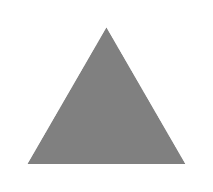
\begin{tikzpicture}
            \fill[gray] (0,0) -- (1,1.73) -- (2,0) -- cycle;
        \end{tikzpicture}
       \item 
\begin{tikzpicture}
            \fill[gray] (0,0) -- (2.2,0) -- (1.85,1.5) -- (0.35,1.5) -- cycle; 
            
        \end{tikzpicture}
        \item  
\begin{tikzpicture}
            \fill[gray] (0,0) rectangle (2,2);
        \end{tikzpicture}
        
        
    \end{enumerate}
    \end{multicols}




The coordinates of the shear center of this cross-section are:
\hfill{[GATE 2022]}
\begin{multicols}{2}
\begin{enumerate}
    \item  $ x = 0,$    $y=3a  $
    \item  $ x=2a,$    $y=2a  $
    \item  $ x =-a,$  $y = 2a  $
    \item  $ x =-2a,$ $y = a  $
\end{enumerate}
\end{multicols}
\item Four different soils are classified as CH, ML, SP, and SW, as per the Unified Soil Classification System. Which one of the following options correctly represents their arrangement in the decreasing order of hydraulic conductivity?

\hfill{[GATE 2022]}\begin{enumerate}
    \begin{multicols}{2}
        \item SW, SP, ML, CH
        \item CH, ML, SP, SW
        \item SP, SW, CH, ML
        \item ML, SP, CH, SW
    \end{multicols}
\end{enumerate}

\vspace{1em}

\item Let $\sigma'_v$ and $\sigma'_h$ denote the effective vertical stress and effective horizontal stress, respectively. Which one of the following conditions must be satisfied for a soil element to reach the failure state under Rankine's passive earth pressure condition?

\hfill{[GATE 2022]}\begin{enumerate}
    \begin{multicols}{2}
        \item $\sigma'_v < \sigma'_h$
        \item $\sigma'_v > \sigma'_h$
        \item $\sigma'_v = \sigma'_h$
        \item $\sigma'_v + \sigma'_h = 0$
    \end{multicols}
\end{enumerate}

\item With respect to fluid flow, match the following in Column X with Column Y:

\begin{center}
\begin{tabular}{|c|c|}
\hline
\textbf{Column X} & \textbf{Column Y} \\
\hline
(P) Viscosity & (I) Mach number \\
(Q) Gravity & (II) Reynolds number \\
(R) Compressibility & (III) Euler number \\
(S) Pressure & (IV) Froude number \\
\hline
\end{tabular}
\end{center}

Which one of the following combinations is correct?

\hfill{[GATE 2022]}\begin{enumerate}
    \begin{multicols}{2}
        \item (P) - (II), (Q) - (IV), (R) - (I), (S) - (III)
        \item (P) - (III), (Q) - (IV), (R) - (I), (S) - (II)
        \item (P) - (IV), (Q) - (II), (R) - (I), (S) - (III)
        \item (P) - (II), (Q) - (IV), (R) - (III), (S) - (I)
    \end{multicols}
\end{enumerate}

\item Let  $ \psi  $ represent soil suction head and  $ K  $ represent hydraulic conductivity of the soil. If the soil moisture content  $ \theta  $ increases, which one of the following statements is \textbf{TRUE}?
\hfill{[GATE 2022]}
\begin{multicols}{2}
\begin{enumerate}
    \item  $ \psi  $ decreases and  $ K  $ increases.
    \item  $ \psi  $ increases and  $ K  $ decreases.
    \item Both  $ \psi  $ and  $ K  $ decrease.
    \item Both  $ \psi  $ and  $ K  $ increase.
\end{enumerate}
\end{multicols}

\item A rectangular channel with Gradually Varied Flow (GVF) has a changing bed slope. If the change is from a steeper slope to a steep slope, the resulting GVF profile is

\hfill{[GATE 2022]}\begin{enumerate}
    \item  $ S_3  $
    \item  $ S_1  $
    \item  $ S_2  $
    \item either  $ S_1  $ or  $ S_2  $, depending on the magnitude of the slopes
\end{enumerate}

\item The total hardness in raw water is 500 $milligram$ per liter as $CaCO_3$. The total hardness of this raw water, expressed in milligram equivalent per liter, is:\\
(Consider the atomic weights of Ca, C, and O as 40 $g/mol$, 12 $g/mol$, and 16 $g/mol$, respectively.)

\hfill{[GATE 2022]}\begin{enumerate}
    \begin{multicols}{4}
        \item 10
        \item 100
        \item 1
        \item 5
    \end{multicols}
\end{enumerate}

\vspace{1em}

\item An aerial photograph is taken from a flight at a height of 3.5 $km$ above mean sea level, using a camera of focal length 152 $mm$. If the average ground elevation is 460 $m$ above mean sea level, then the scale of the photograph is:

\hfill{[GATE 2022]}\begin{enumerate}
    \begin{multicols}{2}
        \item 1 : 20000
        \item 1 : 20
        \item 1 : 100000
        \item 1 : 2800
    \end{multicols}
\end{enumerate}

\item A line between stations P and Q laid on a slope of 1 in 5 was measured as 350 $m$ using a 50 $m$ tape. The tape is known to be short by 0.1 $m$.

The corrected horizontal length (in $m$) of the line PQ will be
\hfill{[GATE 2022]}
\begin{multicols}{4}
\begin{enumerate}
    \item 342.52
    \item 349.30
    \item 356.20
    \item 350.70
\end{enumerate}
\end{multicols}

\item The matrix   $M$  is defined as

\begin{align*}
M = \myvec{1 & 3 \\ 4 & 2 }
\end{align*}

and has eigenvalues 5 and -2. The matrix  $ Q  $ is formed as

\begin{align*}
Q = M^3 - 4M^2 - 2M
\end{align*}

Which of the following is/are the eigenvalue(s) of matrix  $ Q  $?
\hfill{[GATE 2022]}
\begin{multicols}{4}
\begin{enumerate}
    \item 15
    \item 25
    \item -20
    \item -30
\end{enumerate}
\end{multicols}

\item For wastewater coming from a wood pulping industry,Chemical Oxygen Demand(COD) and 5-day Biochemical Oxygen Demand$\brak{BO D_{5}}$ were determined. For this wastewater, which of the following statement(s) is/are correct?\hfill{[GATE 2022]}
\begin{multicols}{4}
\begin{enumerate}
\item $COD > BO D_{5}$
\item $COD \neq BO D_{5}$
\item $COD < BO D_{5}$ 
\item $COD = BO D_{5}$
\end{enumerate}
\end{multicols}

\end{enumerate}


\end{document}
